% --------------------------------------------------------------
% This is all preamble stuff that you don't have to worry about.
% Head down to where it says "Start here"
% --------------------------------------------------------------
 
\documentclass[12pt]{article}
 
\usepackage[margin=1in]{geometry} 
\usepackage{amsmath,amsthm,amssymb}
\usepackage{graphicx}

\newcommand{\N}{\mathbb{N}}
\newcommand{\Z}{\mathbb{Z}}
 
\newenvironment{theorem}[2][Theorem]{\begin{trivlist}
\item[\hskip \labelsep {\bfseries #1}\hskip \labelsep {\bfseries #2.}]}{\end{trivlist}}
\newenvironment{lemma}[2][Lemma]{\begin{trivlist}
\item[\hskip \labelsep {\bfseries #1}\hskip \labelsep {\bfseries #2.}]}{\end{trivlist}}
\newenvironment{exercise}[2][Exercise]{\begin{trivlist}
\item[\hskip \labelsep {\bfseries #1}\hskip \labelsep {\bfseries #2.}]}{\end{trivlist}}
\newenvironment{problem}[2][Problem]{\begin{trivlist}
\item[\hskip \labelsep {\bfseries #1}\hskip \labelsep {\bfseries #2.}]}{\end{trivlist}}
\newenvironment{question}[2][Question]{\begin{trivlist}
\item[\hskip \labelsep {\bfseries #1}\hskip \labelsep {\bfseries #2.}]}{\end{trivlist}}
\newenvironment{corollary}[2][Corollary]{\begin{trivlist}
\item[\hskip \labelsep {\bfseries #1}\hskip \labelsep {\bfseries #2.}]}{\end{trivlist}}
\newenvironment{solution}
  {\begin{proof}[Solution]\renewcommand{\qedsymbol}{}}
  {\end{proof}}

\usepackage{listings}
\usepackage{color}

\definecolor{mygreen}{rgb}{0,0.6,0}
\definecolor{mygray}{rgb}{0.5,0.5,0.5}
\definecolor{mymauve}{rgb}{0.58,0,0.82}

\lstset{ %
  backgroundcolor=\color{white},   % choose the background color; you must add \usepackage{color} or \usepackage{xcolor}
  basicstyle=\footnotesize,        % the size of the fonts that are used for the code
  breakatwhitespace=false,         % sets if automatic breaks should only happen at whitespace
  breaklines=true,                 % sets automatic line breaking
  captionpos=b,                    % sets the caption-position to bottom
  commentstyle=\color{mygreen},    % comment style
  deletekeywords={...},            % if you want to delete keywords from the given language
  escapeinside={\%*}{*)},          % if you want to add LaTeX within your code
  extendedchars=true,              % lets you use non-ASCII characters; for 8-bits encodings only, does not work with UTF-8
  frame=single,                    % adds a frame around the code
  keepspaces=true,                 % keeps spaces in text, useful for keeping indentation of code (possibly needs columns=flexible)
  keywordstyle=\color{blue},       % keyword style
  language=Mathematica,                 % the language of the code
  morekeywords={*,...},            % if you want to add more keywords to the set
  numbers=left,                    % where to put the line-numbers; possible values are (none, left, right)
  numbersep=5pt,                   % how far the line-numbers are from the code
  numberstyle=\tiny\color{mygray}, % the style that is used for the line-numbers
  rulecolor=\color{black},         % if not set, the frame-color may be changed on line-breaks within not-black text (e.g. comments (green here))
  showspaces=false,                % show spaces everywhere adding particular underscores; it overrides 'showstringspaces'
  showstringspaces=false,          % underline spaces within strings only
  showtabs=false,                  % show tabs within strings adding particular underscores
  stepnumber=1,                    % the step between two line-numbers. If it's 1, each line will be numbered
  stringstyle=\color{mymauve},     % string literal style
  tabsize=2,                       % sets default tabsize to 2 spaces
  title=\lstname                   % show the filename of files included with \lstinputlisting; also try caption instead of title
}

\begin{document}


 
% --------------------------------------------------------------
%                         Start here
% --------------------------------------------------------------
 
\title{Homework 1}%replace X with the appropriate number
\author{Maksim Levenal\\ %replace with your name
MAP 4102} %if necessary, replace with your course title
 
\maketitle
 
\begin{problem}{1(a)} %You can use theorem, exercise, problem, or question here.  Modify x.yz to be whatever number you are proving
Compute the transition probability matrix for $X$.
\end{problem}
 
\begin{solution}\ \\

Let $X_n$ be the number of white balls in the left urn at time n. The state space has dimension 6, ranging from 0 white balls in the left urn to all 5 of the white balls in the left urn. We demonstrate how to compute the row entries for rows 0 and 1; the arguments for rows 2, 3 and 4 are similar to that of row 2 and row 5 is similar to that of row 1.

If there are 0 white balls in the left urn then all of the black balls are in the left urn. Hence the left urn will transition to containing 1 white ball w.p. 1 and all other transitions have probability 0. Transitions from state  5 are the obverse. If there is 1 white ball in the left urn then there are 4 black balls in the left urn, 1 black ball in the right urn, and 4 white balls in the right urn. The probability of transitioning to state 0 is that of choosing the one white ball in the left urn and choosing the one black ball in the right urn, 

$$ \frac{1}{5} \times \frac{1}{5} = \frac{1}{25}.$$

\noindent The probability of transitioning to the state wherein the left urn contains 2 balls is the complement of choosing the exceptional ball in each urn,

$$ \frac{4}{5} \times \frac{4}{5} = \frac{16}{25}.$$

\noindent The probability of returning to state 1, from state 1, is the sum of the probabilities of swapping white balls or black balls between both urns,

$$ \frac{4}{5} \times \frac{1}{5} + \frac{1}{5} \times \frac{4}{5}= \frac{8}{25}.$$

Hence the transition matrix is 

$$\frac{1}{25}\begin{pmatrix} 
	  & 25 &    &    &    &  \\ 
	1 & 8  & 16 &    &    &  \\
	  & 4  & 12 & 9  &    &  \\ 
	  &    & 9  & 12 & 4  &  \\
	  &    &    & 16 & 8  & 1\\
	  &    &    &    & 25 & 
\end{pmatrix}$$
%Note 1: The * tells LaTeX not to number the lines.  If you remove the *, be sure to remove it below, too.
%Note 2: Inside the align environment, you do not want to use $-signs.  The reason for this is that this is already a math environment. This is why we have to include \text{} around any text inside the align environment.

\end{solution}

\begin{problem}{1(b)} %You can use theorem, exercise, problem, or question here.  Modify x.yz to be whatever number you are proving
Does this Markov chain have a stationary distribution? If so, compute it.

\end{problem}
 
\begin{solution}\ \\ 

The Markov chain is irreducible because all of the classes communicate (and hence positive recurrent but that's irrelevant presently). It's aperiodic, to wit ergodic, manifestly so because state 2 can transition to state 2 with probability .32 in 1 step, hence it has a unique stationary distribution. To find $\pi$ we set up the linear system $\pi = \pi \mathbf{P}$ with the added constraint that $\sum_{j \in S}\pi_j = 1$ and solve for $\pi$. To effect the constraint we can replace the last column in the transition matrix with 1s and replace the last entry in the output vector also with a 1. 

\begin{align*}
\begin{pmatrix} 
			\pi_0  \\ 
			\pi_1  \\
			\pi_2  \\ 
			\pi_3  \\
			\pi_4  \\ 
			1  \\
			\end{pmatrix}
			& = \frac{1}{25}\begin{pmatrix} 
			\pi_0  \\ 
			\pi_1  \\
			\pi_2  \\ 
			\pi_3  \\
			\pi_4  \\ 
			\pi_5  \\
			\end{pmatrix}
			\begin{pmatrix} 
			  & 25 &    &    &    & 1 \\ 
			1 & 8  & 16 &    &    & 1\\
			  & 4  & 12 & 9  &    & 1 \\ 
			  &    & 9  & 12 & 4  & 1 \\
			  &    &    & 16 & 8  & 1\\
			  &    &    &    & 25 & 1
			\end{pmatrix} \\
\end{align*}
Using the Mathematica code : \\

\begin{lstlisting}[frame=single]  
P = (1/25 {{0, 25, 0, 0, 0, 25}, 
		       {1, 8, 16, 0, 0, 25}, 
		       {0, 4, 12, 9, 0, 25},
           {0, 0, 9, 12, 4, 25}, 
           {0, 0, 0, 16, 8, 25}, 
           {0, 0, 0, 0, 25, 25}})
  
p = {p0, p1, p2, p3, p4}  

Solve[p.P == {p0, p1, p2, p3, 1}]
\end{lstlisting}
yields $\pi = \left( \frac{1}{252}, \frac{25}{252}, \frac{25}{63}, \frac{25}{63}, \frac{25}{252}, \frac{1}{252} \right)$

\end{solution} 

\begin{problem}{2(a)} %You can use theorem, exercise, problem, or question here.  Modify x.yz to be whatever number you are proving
What is the state space of this Markov Chain and what is the transition matrix P?

\end{problem}

\begin{solution}\ \\

The state space is $\{0,1,2,3,4\}$ newspapers in the pile in the evening. It is impossible for there to be five or more papers in in the pile because Mr. Smith would have recycled them in the afternoon. The transition matrix $P$ is

$$\begin{pmatrix} 
	.33 & .66 &     &      &      \\ 
	.33 &     & .66 &      &      \\
	.33 &     &     & .66  &      \\ 
	.33 &     &     &      & .66  \\
	1   &     &     &      &      \\  
\end{pmatrix}$$
\end{solution}

\begin{problem}{2(b)} %You can use theorem, exercise, problem, or question here.  Modify x.yz to be whatever number you are proving
What is the probability there are 0 papers in the pile if 2 evenings ago there were 3?

\end{problem}

\begin{solution}\ \\

This is calculated by applying $ P^2 $ to the initial distribution $ (0,0,0,1,0) $ . $P^2$ is computed using the Mathematica code : \\

\begin{lstlisting}[frame=single]  
P = ({
      {.33, .66,    0,   0,   0},
      {.33,   0,  .66,   0,   0},
   	  {.33,   0,    0, .66,   0},
      {.33,   0,    0,   0, .66},
      {  1,   0,    0,   0,   0}
     })
  
MatrixPower[P,2]
\end{lstlisting}Hence 

\begin{align*}
\begin{pmatrix}
0 & 0 &  0   &  1    & 0
\end{pmatrix}\times
\begin{pmatrix} 
	.33 & .66 &     &      &      \\ 
	.33 &     & .66 &      &      \\
	.33 &     &     & .66  &      \\ 
	.33 &     &     &      & .66  \\
	1   &     &     &      &      \\  
\end{pmatrix}^2 & = \begin{pmatrix}
0 & 0 &  0   &  1    & 0
\end{pmatrix}\times
\begin{pmatrix} 
 0.33 & 0.22 & 0.44 & 0. & 0. \\
 0.33 & 0.22 & 0. & 0.44 & 0. \\
 0.33 & 0.22 & 0. & 0. & 0.44 \\
 0.77 & 0.22 & 0. & 0. & 0. \\
 0.33 & 0.66 & 0. & 0. & 0. \\
\end{pmatrix}\\
& = \begin{pmatrix}
.77 & .23 &  0   &  0    & 0
\end{pmatrix}
\end{align*}
So there is a .77 probability that there 0 papers in the pile on the second evening.
\end{solution}


\begin{problem}{2(c)} %You can use theorem, exercise, problem, or question here.  Modify x.yz to be whatever number you are proving
Argue, via numerical experimentation, whether there exists a limiting distribution of
papers in the pile.


\end{problem}

\begin{solution}\ \\

Using the Mathematica code \\

\begin{lstlisting}[frame=single]  
P = ({
      {.33, .66,    0,   0,   0},
      {.33,   0,  .66,   0,   0},
   	  {.33,   0,    0, .66,   0},
      {.33,   0,    0,   0, .66},
      {  1,   0,    0,   0,   0}
     })
  
MatrixPower[P,1000]
\end{lstlisting}generates the asymptotic transition matrix 

$$\begin{pmatrix} 
 0.38 & 0.26 & 0.17 & 0.11 & 0.08 \\
 0.38 & 0.26 & 0.17 & 0.11 & 0.08 \\
 0.38 & 0.26 & 0.17 & 0.11 & 0.08 \\
 0.38 & 0.26 & 0.17 & 0.11 & 0.08 \\
 0.38 & 0.26 & 0.17 & 0.11 & 0.08 \\
\end{pmatrix}
$$
So the limiting distribution is $ (0.38, 0.26, 0.17, 0.11, 0.08) $.
\end{solution}

\begin{problem}{3(a)} %You can use theorem, exercise, problem, or question here.  Modify x.yz to be whatever number you are proving
Draw a flow diagram of this Markov Chain and classify all of its states as stationary or
recurrent.
\end{problem}
\begin{solution}\ \\

\begin{center}
	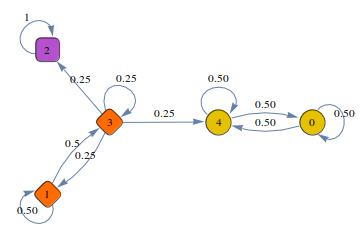
\includegraphics[scale=.7]{transition_diagram.jpg}
\end{center}

States $1$ and $3$ are transient. To see this note that if $X_0 = 3$ then there is a $.25$ probability of the chain going to state $2$ and being absorbed, so $P_3(T_1 = \infty) \geq p(3,2) = .25 > 0$. Further since state 1 is in the same communicating class as state 3 it too is transient (because transience is a class property). State 3 is trivially recurrent. State 4 and 0 are recurrent because they comprise an irreducible closed class.
\end{solution}

\begin{problem}{3(b)} %You can use theorem, exercise, problem, or question here.  Modify x.yz to be whatever number you are proving
Find all of its stationary distributions.
\end{problem}
\begin{solution}\ \\

There are 3 stationary distributions. One for each closed recurrent class and one that is a linear combination of them that represents starting in the transient class, with coefficients being the relative probabilities of transitioning to either recurrent class from the transient class.

We can find the stationary distributions of the recurrent classes by performing eigenvalue decomposition and identifying the eigenvectors corresponding to the eigenvalue 1. To compute the left eigenvectors of the transition matrix we compute the right eigenvectors of the transpose. Using the Mathematica code \\
\lstset{language=Matlab}
\begin{lstlisting}[frame=single]  
P = ({
      {.5,   0,    0,   0,  .5},
      { 0,  .5,    0,  .5,   0},
   	  { 0,   0,    1,   0,   0},
      { 0, .25,  .25, .25, .25},
      {.5,   0,    0,   0,  .5}
     })

Eigensystem[Transpose[P]]
\end{lstlisting}

\noindent we get that the pertinent eigen-row-vectors are $(0,0,1,0,0)$ and $(0.654, 0, 0.382, 0, 0.654)$. Orthonormalizing yields $(0,0,1,0,0)$ and $(0.5, 0, 0, 0, 0.5)$. There is one more stationary distribution, that due to starting in the transient class and evolving to one of the recurrent classes. It is the linear combination of both of the 2 aforementioned eigenvectors with weights equal to the probability associated with ending up in that recurrent class, hence by inspection of the diagram, it is 

$$
\frac{.25}{.25+.25}(0,0,1,0,0) + \frac{.25}{.25+.25}(0.5, 0, 0, 0, 0.5) = (.25,0,.5,0,.25)
$$


\end{solution}

\begin{problem}{3(c)} %You can use theorem, exercise, problem, or question here.  Modify x.yz to be whatever number you are proving
Suppose we start in state A. In the long run, what percentage of the time do we spend
in state A?

\end{problem}

\begin{solution}\ \\

$50\% $ because $A$ is in a closed recurrent class and the limiting distribution for that recurrent class dictates that transitioning from $A \rightarrow A$ and transitioning $A \rightarrow D$, and vice-versa, each happen with probability $ .5$ .

\end{solution}

\begin{problem}{3(d)} %You can use theorem, exercise, problem, or question here.  Modify x.yz to be whatever number you are proving
Suppose we start in state C. In the long run, what percentage of the time do we spend
in state A?

\end{problem}
\begin{solution}\ \\

$0\%$ because $C$ is in a closed recurrent class of its own.

\end{solution}

\begin{problem}{3(e)} %You can use theorem, exercise, problem, or question here.  Modify x.yz to be whatever number you are proving
Suppose we start in state B. In the long run, what percentage of the time do we spend
in state A?

\end{problem}
\begin{solution}\ \\

$.25$ because there are 2 recurrent classes, that of $\{C\}$ and that of $\{A,E\}$ and the chance of transitioning from $B$'s class to $A$'s is relatively .5 and then the chance of being in $A$ after transitioning to $A$'s class is again .5. So the composite probability is $.5 \times .5$.

\end{solution}

\begin{problem}{3(f)} %You can use theorem, exercise, problem, or question here.  Modify x.yz to be whatever number you are proving
Why did I have to change the wording of the question in the last item?


\end{problem}
\begin{solution}\ \\

Because there is not a unique limiting distribution so there is a non-vanishing probability that the Markov chain doesn't end up in $A$ at all. So speaking of the proportion of time spent in $A$ is semantically incorrect. 
\end{solution}


\begin{problem}{5} %You can use theorem, exercise, problem, or question here.  Modify x.yz to be whatever number you are proving
Prove that if we make the random walk “lazy”, in the sense that we always give the walker a probability q of not moving, then $\pi$ is also a stationary distribution of the lazy random walk.
\end{problem}
\begin{solution}\ \\

Let $\pi$ be the limiting distribution of the strict random walk, i.e. $\pi\mathbf{P}=\pi$. The "lazy" random walk is related to the strict random walk as such: $\mathbf{P_\ell} = \mathbf{P}(1-q) + \mathbf{I}q$ where $I$ is the identity matrix. This is the case because if the chain does not transition with probability $q$ then it \textit{does} transition with probability $(1-q)$ and whether it transition up or down is conditional on it transitioning at all, hence the "step" probabilities are $p_{ij}\times(1-q)$. That $\pi$ is a limiting distribution follows immediately: $\pi \mathbf{P_\ell} = \pi \mathbf{P} (1-q) + \pi \mathbf{I} q = \pi(1-q) + \pi q = \pi$.

\end{solution}
% --------------------------------------------------------------
%     You don't have to mess with anything below this line.
% --------------------------------------------------------------
 
\end{document}
\begin{align*}
\sum_{i=1}^{k+1}i & = \left(\sum_{i=1}^{k}i\right) +(k+1)\\ 
& = \frac{k(k+1)}{2}+k+1 & (\text{by inductive hypothesis})\\
& = \frac{k(k+1)+2(k+1)}{2}\\
& = \frac{(k+1)(k+2)}{2}\\
& = \frac{(k+1)((k+1)+1)}{2}.
\end{align*}